\documentclass[a4paper,11pt]{article}
\oddsidemargin 0.0cm  
\evensidemargin 0.0cm  
\textwidth 17cm 
\topmargin -1cm 
\textheight 23.5cm
\usepackage{graphicx}
\usepackage{float} 
\usepackage{multimedia}
\usepackage{amsmath,amssymb}
\usepackage{listings}
\usepackage{graphicx} % Allows including images
\usepackage{booktabs} % Allows the use of \toprule, \midrule and \bottomrule in tables
\usepackage[nottoc, notlof, notlot]{tocbibind}
\usepackage{scrextend}
\usepackage{amsfonts}
\usepackage{amsmath,bm}
\usepackage{graphicx}
\usepackage{hyperref}
\usepackage[round]{natbib}
\lstset{
  numbers=left,   
  firstnumber=1,
  numberfirstline=true,
  language=C, 
  frame=L
  } 



\bibliographystyle{plain}


\title{Internship: Inverse Procedural Generation of Geological Stories}
\author{Maxime Garcia}
\date{\today}

\begin{document}
\maketitle
\section{General Overview}

Here we will present our first method to tackle the problem of proposing a panel of plausible animations giving geological restoration as final state from a 2D input slice. 
The main idea of our methods is to map a mass spring system on each block (section between two or several faults) of the slice and simulate a extension by freezing the physics of several blocks at each time step and let the others move as they should given geological events. The output of our method we will a series of inbetween VGC which will be played on VPaint.\\\\
The first step of our method is to draw the 2D slice using VPaint which allow the user to do it pretty quickly.
This drawing will highlight all the different blocks which are contained in the slice.
In addition the VPaint drawing will show all the different layers of each block and faults. Additionnal information such as erosion lines can be added. \\\\
After drawing our section in VPaint we will read the .vec file in our GeoPaint editor in order to add all the necessary information about our section such as the layers' materials containing crutial information (density, age, etc...) or even  additionnal information about faults and erosion lines. This information will allow us to run the animation over our section.
Indeed once the geo editing is finished we will gather all the information into one format (.geo) and will use it to describe our slice and animate it.\\\\
The first step for animating is mapping a mass-spring system into each block. Then we have to solve the restoration problem at a geological point of view, that is to say build the first story tree and find a method to propose which event can happen at each node.\\\\
As the first proposed story tree is computed fully automaticaly it may not show the most plausible result that's why we propose the user to choose events a list of plausible geological events at each node.
This way the user can construct all the plausible stories he wants.

\section{General structure}
One important matter in our model is to choose carefully the representation of our slices as it will affect how we will animate it.
We choose one possible representation of a geological slice but we are aware that some part of this structure can be modified through the project progression.\\\\
Similary to the drawing a slice is composed of blocks, faults and erosion lines. It also contains a list of all the materials composing the different layers.This list will be usefull when we want to see if one material disappeared from one block. Each blocks is composed of layers and interlayers lines. Knowing all the interlayers is important to link the layer mapping together (see Animation Model section).\\\\
Each block contains a list of the materials composing its layers. Like said abbove we will compair it to the slice material to take into account erosion effect which cause layers to disappear. \\\\
Each layer contains its interlayers,left and right sides and also its corners which are important for linking blocks together during the animation. The layer contains also its material which gives a lot information for the animation (density, friction, erosion speed, sedimentation speed). 
In fact this information will be taken into consideration inside the mass spring system attached to the layer.
Each fault contains each line composing it. Sub faults which we know that came after an other can be added.


\section{Animation Model}

Like mentionned above the animation will be done by mapping a mass-spring system on each block. In fact it is more accurate to say that mass-spring system are mapped on layers instead of blocks. We proceed this way to take into account each layer orientation in the mapping as it is mapped according to layer's borders gradients. Considering that each layer is a rectangle that underwent some deformations the mapping will be done following the steps:	\\\\		
\indent	- First we have to put the masses both at the layer border but also inside it.\\\\
\indent	- We put the masses on the borders in an uniform way.\\\\
\indent	- We put the masses inside the layer: to do so we have two solutions:\\\\
\indent \indent	- Compute hermite curve between each pair mass of the two interlayer and place particles uniformly on those curves.\\\\
\indent \indent	- Compute the intersections between the previous hermite curves and the  one coming from each pair mass of the two sides and place particles at those intersections.\\\\
	Even if the second solution might show better results that the first one we have chance that the curve comming from the sides might be not inside the layer due to big deformation making the layer non convex. \\With the first solution this problem is unlikely to occur because of the type of the deformations. In either case the hermite curves be created using a mass pair and the gradient of the broder at each extremity as tangents. This way the layer will tend to transform back to a rectangle shape.\\\\
\indent	- Link particles with springs. \\We divide springs into 5 categories like described in \citep{cloth}: Vertical, Horizontal, DownShear, UpShear and Flexion. Adding flexion spring show better results in terms of shape preservation and breaking prevention. The resulting network looks like:\\
	
	\begin{figure}[H]
	\centering
	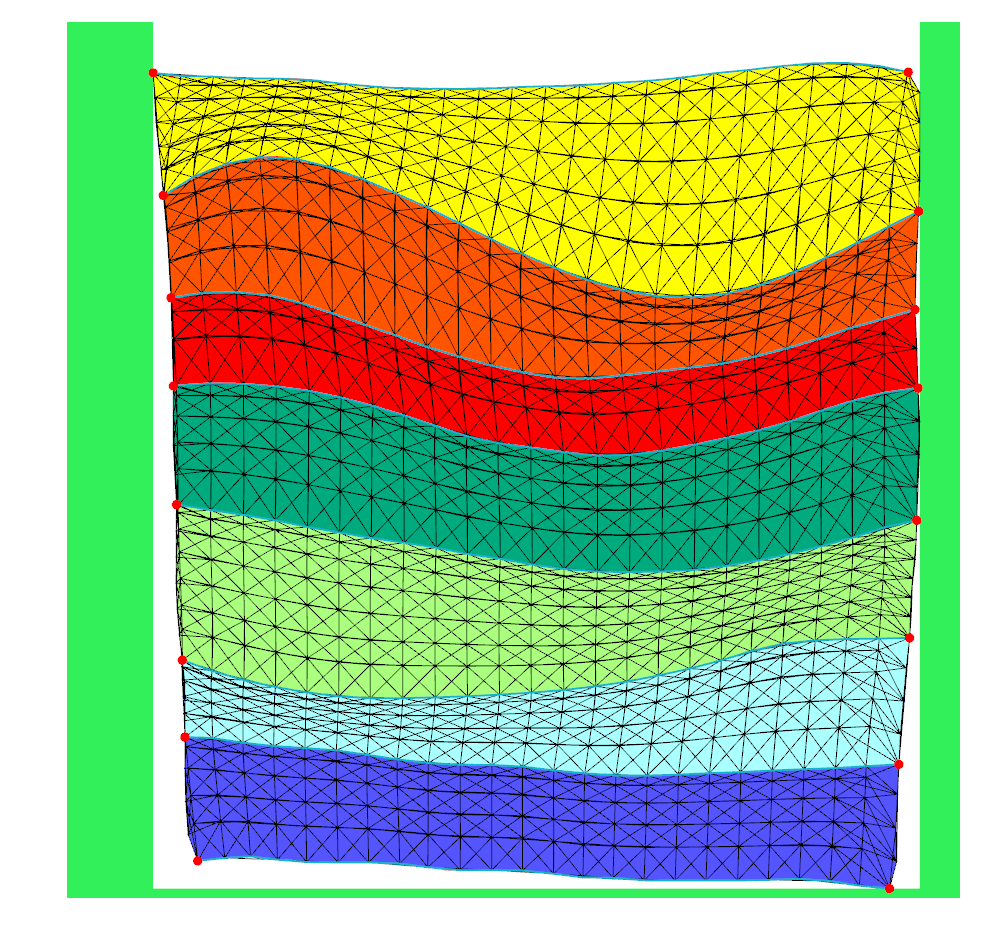
\includegraphics[scale=0.5]{springMapping.png}
	\caption{Mass-Spring Mapping on a layer. In purple: interlayers. In white: sides}
	\end{figure}
	
	
\indent	- The springs we use will also have a torsion resistance in order to accentuate the shape change of the layer.\\\\
In terms of physical equations for a single mass spring system we use the implicit euler scheme and algorithm descibed in \citep{caltech}. We use this scheme instead of an explicit one because it is proven to be more stable with big time step ($dt = 0.02$).\\\\ 
Each particle has the same mass $m$ and possesses at step $n$:\\\\
\indent	- A position  $x_i^n$\\\\
\indent	- A speed $v_i^n$ \\\\\
\indent	- Applied forces $F_i^n$ (containing filtered, corrected and external forces).\\\\
At each time step we will solve the second Newton's law:\\

\begin{align}
	v_i^{n+1} &= v_i^n + F_i^{n+1} \frac{dt}{m}\\
	x_i^{n+1} &= x_i^n + v_i^{n+1} dt 
\end{align}

with:

\begin{equation}
F_i^{n+1} = - \sum\limits_{j|(i,j)\in Edges} k_{ij}(x_i - x_j) + k_{ij}l_{ij}^0\frac{(x_i - x_j)}{||(x_i - x_j)||}
\end{equation}


For each particle we want to integrate the above equations. The problem is that we don't know the forces at step $n + 1$ as we don't know the position of the particles at this step. That is why we use a first order approximation to solve the problem at step $n + 1$:

\begin{equation}
	F^{n+1} = F^n + \frac{\partial F}{\partial x}(x^{n+1} - x^n)
\end{equation}

\noindent Thus we need to compute $H =  \frac{\partial F}{\partial x}$ which is the Jacobian of $F$.\\\\
\noindent By using (1) and (4) we have the following result:
\begin{align*}
	(x^{n+1} - x^n) &= (v^n + (v^{n+1} - v^n))dt \\
	(v^{n+1} - v^n) &= (I - \frac{dt^2}{m}H)^{-1}(F^n + dt H v^n)\frac{dt}{m}
\end{align*}

We now have approximated our equations into a solvable system and we can notice that an additionnal force came from this approximation $dt H v^n$ . It is an implicit viscosity that takes into account the movement of the neighbouring particles.
Consequently we have for each particle $i$ a new force:

\begin{equation}
\tilde{F_i} = k dt \sum\limits_{j|(i,j)\in Edges}(v_j - v_i)
\end{equation}


The last thing to compute is $H$. Like in \citep{caltech} we will approximate $H$ by just integrating the linear part of the elastic force which is equal to:

\begin{equation}
F_{(i,j)} = -k_{ij}(x_i - x_j) + k_{ij}l_{ij}^0\frac{(x_i - x_j)}{||(x_i - x_j)||}
\end{equation}

If $H$ represents only the Jacobian of $F = -k_{ij}(x_i - x_j)$ it has the form:\\
\begin{center}
$
\left\{
\begin{array}{ll}
H_{ij} &= k_{ij} if i \neq j \\
H_{ii} &= -\sum\limits_{j \neq i}k_{ij}
\end{array}
\right.
$
\end{center}

Integrating only the linear part implies that we will have some error at the end of the integration. However we can notice that the non linear part $k_{ij}l_{ij}^0\frac{(x_i - x_j)}{||(x_i - x_j)||}$ has a constant magnitude during the simulation between two steps, so this force just implies a rotation that we will compensiate with another force. Thus we will correct the angular momentum $\delta T$ introduced by this method by adding correcting forces:
\begin{align*}
\delta T &= \sum\limits_{i=1}^n (x_G - x_i)\wedge F_i^{filtered} \\
F_i^{corrected} &= (x_G - x_i)\wedge \delta T dt
\end{align*}

with:
\begin{equation}
F_i^{filtered} = \sum\limits_{i=1}^n F_{ji}W_{ij}
\end{equation}

However in our case the equilibrum length of the springs will change over time creating an error in the angular momentum but we will try compensating this with torsion forces.\\\\

Finally we add torsion forces as external forces (along with gravity) because it is a non linear force and we can't integrate it:

\begin{equation}
F_{ij}^{torsion} = -k_{torsion}\Delta \theta \vec{n}
\end{equation}

with $\Delta \theta$ being the angle between a unit vector depending on the spring type (Vertical, Horizontal, DownShear or UpShear) and the vector $x_i - x_j$. $\vec{n}$ is the normal vector to $x_i - x_j$ pointing toward the unit vector.\\\\
Having this physical structure we will simulate extension and take into account geological features. For the moment we assume that the density and the spring stiffnesses (elastic and torsion) are proportionnal. The friction coefficient will directly be taken into account in the collision computation between faults and particles. As for erosion and sedimentation we will add or remove partcle in the mass-spring system to simulate those events.\\\\
Regarding the extension simulation we will first pull the side where the extension has to occur. This is known before simulating because it is provided by the user. At each time step we will freeze the animation of all the blocks, translate them toward extension apply the physics only to the blocks which are considered to move. The blocks moving undergo either discrete geological event (such as fault) or/and continuous event (erosion or sedimentation). When solving fault apparition we have to stick blocks together. This will be done by attaching corners of the layers when the matching ones are near each other enough. When all the corners are matched we have a new block where we must recompute a new mass spring system.\\\\
Computing a mass spring system can take some time (few seconds for big systems) and can be noticable especially during block fusion but that is not a problem because the goal of the project is to record at each time step the result of our simulation as an inbetween vac which can be played fluently.\\\\

\bibliography{pfe.bib}

\end{document} 